\documentclass[aspectratio=169]{beamer}
\usepackage{standalone}
\usepackage{amsmath}
\usepackage{bm}

\usepackage{stmaryrd}
\usepackage{listings}
\usepackage{bussproofs}

\usepackage[hyperref=auto,style=alphabetic,backend=bibtex]{biblatex}
\addbibresource{kwarcpubs.bib}
\addbibresource{extpubs.bib}
\addbibresource{extcrossrefs.bib}
\addbibresource{bib.bib}
\usepackage{appendixnumberbeamer}
\usepackage{tikz}
\usepackage{tikz-qtree}
\usetikzlibrary{arrows.meta}

\usetheme{Pittsburgh}
% \setbeamertemplate{footline}[frame number]
\setbeamertemplate{footline}{\hfill\insertframenumber\,/\,\inserttotalframenumber\quad\strut}
\setbeamertemplate{navigation symbols}{}
\usecolortheme{beaver}
\setbeamertemplate{frametitle}[default][left]
% \setbeamersize{text margin left=3em}

\usepackage{utils/colors}
\usepackage[forbeamer]{utils/basic}
\usepackage{utils/operators}
\usepackage{utils/mylstmisc}
\usepackage{utils/lstmmt}

% \lstset{basicstyle=\ttfamily}
% \lstset{commentstyle=\itshape\color{commentfont}}
% \definecolor{codegray}{rgb}{0.9,0.9,0.9}
\lstset{basicstyle=\sf,columns=fullflexible}
\lstset{numberstyle=\tiny}
\lstset{language={[LaTeX]TeX}}
\lstset{literate=--1}

\title{Semantic Authoring in a Flexiformal Context --- Bulk Annotation of Rigorous Documents}

\author{Michael Kohlhase, \bf Jan Frederik Schaefer}
\institute{FAU Erlangen-N\"urnberg}
\date{18\textsuperscript{th} Conference on Intelligent Computer Mathematics\\Brasilia, Brazil\\October 8, 2025}

        

\begin{document}

\frame\titlepage


\begin{frame}
    \frametitle{ALeA Ecosystem}
    \begin{columns}
        \column{0.4\textwidth}
        An adaptive learning assistant that
        \begin{itemize}
            \item tracks learner's progress,
            \item suggests practice problems,
            \item is powered by semantic annotations
        \end{itemize}
        \column{0.6\textwidth}
        \centering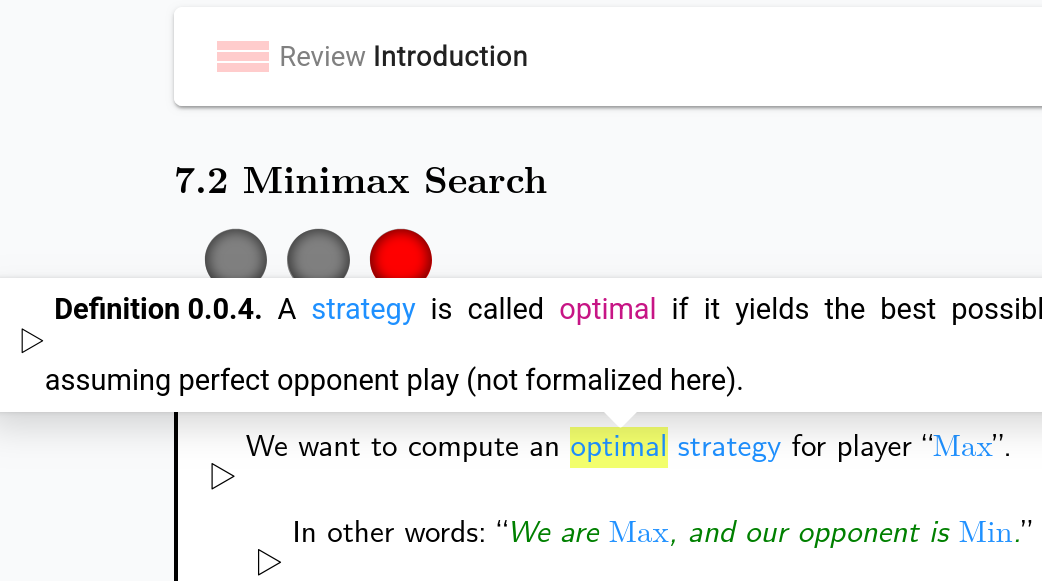
\includegraphics[width=\textwidth]{alea1.png}
    \end{columns}
    \vspace{2em}\par\centering
        {\bf More semantic annotations $\bm\leadsto$ better service}
\end{frame}

\begin{frame}[fragile]
    \frametitle{The Cost of Adoption}
    % {\centering\bf More semantic annotations $\bm\leadsto$ better service}

    % horizontal line
    % \noindent\rule{\textwidth}{0.8pt}
    \lstset{escapeinside={<*}{*>}}
%     \begin{lstlisting}
%     \textbf{Note:} Depth-limited minimax requires an
%     evaluation for every cut-off state $s$.
%     If $s$ is terminal, we use its utility, and otherwise an estimate.
%     \end{lstlisting}
    \def\h#1{\colorbox{yellow!50!red!70}{#1}}
    \begin{lstlisting}
    <*\only<2->{\h{\textbackslash usemodule[courses/FAU/AI/course]\{search/slides?id-search\}}}*>
    <*\only<3->{\h{\textbackslash usemodule[courses/FAU/AI/course]\{game-play/slides?minimax-algo\}}}*>
    \textbf{Note:} <*\only<2->{\h{\textbackslash sr\{depth limit\}\{}}*>Depth-limited<*\only<2->{\h{\}}}*> <*\only<3->{\h{\textbackslash sn\{}}*>minimax<*\only<3->{\h{\}}}*>
    requires an evaluation for every cut-off state $s$.
    If $s$ is terminal, we use its utility, and otherwise an estimate.
    \end{lstlisting}

    \onslide<4->{
        \noindent\rule{\textwidth}{0.8pt}
        \vspace{0.5em}
        \textbf{This is difficult}
        \begin{itemize}
            \item $\ge 5\,400$ concepts in domain model\com{cannot remember them}
            \item manual annotation very tedious, especially for novices
            \item many annotations needed for a lecture\com{estimate: 10\,000}
        \end{itemize}
    }
    \onslide<5>{
        \vspace{0.5em}
        \textbf{Obvious idea: Have tool support $\bm\leadsto$ Snify (\textbackslash sn-ify)}
    }
\end{frame}

\begin{frame}
    \frametitle{Number of Annotations}
    \centering
    \includegraphics{annocounts.pdf}
\end{frame}

\begin{frame}[fragile]
    \frametitle{Making a Catalog}
    \lstset{escapeinside={<*}{*>}}
    \def\h#1{\colorbox{yellow!50!red!70}{#1}}
    \begin{lstlisting}
    \usemodule[courses/FAU/AI/course]{search/slides?id-search}
    \usemodule[courses/FAU/AI/course]{game-play/slides?minimax-algo}
    \textbf{Note:} <*{\h{\textbackslash sr\{depth limit\}\{Depth-limited\}}}*> <*{\h{\textbackslash sn\{minimax\}}}*>
    requires an evaluation for every cut-off state $s$.
    If $s$ is terminal, we use its utility, and otherwise an estimate.
    \end{lstlisting}

    % \pause
    \noindent\rule{\textwidth}{0.8pt}
    \begin{itemize}
        \item Collect symbol verbalizations from annotations
        \item Also for other languages (\textbackslash sr\{depth limit\}\{tiefenbeschr\"ankt\})
        \item Use stemmer to deal with inflections:
            \begin{itemize}
                \item ``limit'' $\mapsto$ ``limit''
                \item ``limits'' $\mapsto$ ``limit''
                \item ``limited'' $\mapsto$ ``limit''
            \end{itemize}
    \end{itemize}
    
\end{frame}


\begin{frame}
    \frametitle{Snify}
    % Simple tool for sTeX bulk annotation:
    {\centering\it\large Source-based, incremental, interactive, fine-grained annotation workflow\par\vspace{1.5em}}
    \begin{itemize}
        \item Iterates over source files
        \item Suggests annotations to user\com{
            select annotation instead of remembering and entering it
            }
        \item Inspired by traditional spell-checkers (e.g. ispell/aspell/...)
        \item Snify implementation:
            \begin{itemize}
                \item A workflow experiment
                \item Very useful in practice
                \item Simple command line interface
            \end{itemize}
    \end{itemize}
\end{frame}

\begin{frame}
    \frametitle{Demo}
\end{frame}

% \begin{frame}[fragile]
%     \frametitle{The Catalog}
%     \lstset{escapeinside={<*}{*>}}
%     \def\h#1{\colorbox{yellow!70!red!70}{#1}}
%     \begin{lstlisting}
% ... is called a \definame{<*\h{goal state}*>} (or \definiendum{goal state}{<*\h{terminal state}*>}).
%     \end{lstlisting}
%     \[\downarrow\text{\bf Extract verbalizations}\]
%     \vspace{-1.5em}
%     \begin{itemize}
%         \item {\color{blue}\verb|https://...search problem&s=goal state|} $\leftrightsquigarrow$ ``goal state'', ``terminal state'', \pause ``goal'', ``end state'', ``terminal'', ``terminal positions''
%         \item {\color{blue}\verb|https://...grammar&s=terminal symbol|} $\leftrightsquigarrow$ ``terminal symbol'', ``terminal''
%         \item {\color{blue}\verb|https://...terminal&s=terminal|} $\leftrightsquigarrow$ ``computer terminal'', ``terminal''
%         \item \textellipsis
%     \end{itemize}
%     \pause
%     \par\vspace{1em}
%     \begin{columns}
%         \column{0.1\textwidth}
%         \ 
%         \column{0.3\textwidth}
%     \textbf{Using a stemmer to manage inflection:}
%         \column{0.6\textwidth}
%         \begin{tikzpicture}
%         \node (a) at (0, 0) {termin};
%         \node (b) at ( 2.5, -1) {terminal};
%         \node (c) at ( 2.5,  1) {terminals};
%         \node (d) at (-2.5,  1) {terminate};
%         \node (e) at (-2.5, -1) {terminating};
%         \draw[-Stealth,thick] (b) to[sloped] node[above] {stem} (a);
%         \draw[-Stealth,thick] (c) to[sloped] node[above] {stem} (a);
%         \draw[-Stealth,thick] (d) to[sloped] node[above] {stem} (a);
%         \draw[-Stealth,thick] (e) to[sloped] node[above] {stem} (a);
%     \end{tikzpicture}
%     \end{columns}
% \end{frame}



\begin{frame}
    \frametitle{Beyond the Core Idea}
    \textbf{Also needed to make this work:}
    \begin{itemize}
        \item Support multiple language
        \item Add new imports, remove redundant imports
        \item Only annotate text (not macros, formulae, code, \textellipsis)
    \end{itemize}

    \vspace{1em}
    \textbf{+ various productivity features:}
    \begin{itemize}
        \item Undo/Redo
        \item Edit in editor
        \item Select symbol that is not suggested
        \item Permanently skip word in document/everywhere
        \item Explain why a symbol is suggested/how it is imported
        \item Focus mode
        \item ...
    \end{itemize}
\end{frame}

\begin{frame}
    \frametitle{Evaluation}
    \textbf{Effect:}
    \begin{itemize}
        \item Productivity gain over sTeX IDE: $3\times$ -- $13\times$
        \item Higher annotation density
        \item Used by most sTeX annotators
        \item Has been used for estimated 10\,000 annotations, possibly 20\,000
    \end{itemize}

    \vspace{1em}
    \textbf{Limitations:}
    \begin{itemize}
        \item Catalog must be reasonably complete for document language
        \item Only words in the catalog are offered $\leadsto$ less awareness of gaps in domain model?
        \item Does not support annotation while writing
        \item Only supports annotation of symbol references in text\com{no formulae, no metadata, \textellipsis}
    \end{itemize}
\end{frame}

\begin{frame}
    \frametitle{Side Effect: Debugging the Domain Model}
    Different perspective on domain model with
    focus on what we care about right now.

    Snify helps detect e.g.:
    \begin{itemize}
        \item Gaps in the domain model
        \item Duplicate symbols
        \item Unnecessary dependencies
    \end{itemize}

    % TODO: screenshots
\end{frame}


\begin{frame}
    \frametitle{Semantic Authoring}
    \begin{tabular}{r l l l}
        & \textbf{Informal Authoring} & \textbf{Semantic Authoring} & \textbf{Formal Authoring} \\[0.3em]
        Example & informal \LaTeX & sTeX & computer code \\[0.3em]
        \pause
        Dom. model & in head/literature & glossary & libraries \\[0.3em]
        \pause
        People & mathematicians & we & formalizers \\[0.3em]
        \pause
        Reuse & limited & more desirable \& possible & all the time \\[0.3em]
        \pause
        % Tools & spell/grammar checker & \begin{tabular}c\textbf{?}\end{tabular} & IDE (refactoring, \textellipsis) \\[0.3em]
        Tools & spell/grammar checker & \large\textbf{?} & IDE (refactoring, \textellipsis) \\[0.3em]
    \end{tabular}

    \pause
    \vspace{1.5em}
    \textbf{Semantic authoring tool support:}
    \begin{itemize}
        \item spell/grammar checking \com{like informal authoring}
        \item IDE functionality (e.g.\ refactoring symbol names) \com{like formal authoring}
        \item need tools that combine both aspects \com{like Snify}
    \end{itemize}
\end{frame}

\begin{frame}[fragile]
    \frametitle{Design Space of Semantic Authoring}
    \def\h#1{\only<1>{#1}\only<2>{\colorbox{yellow!50!red!70}{#1}}}
    % \def\h#1{#1}
    \begin{itemize}
        \item \h{Text} vs formulae vs metadata\com{or combination?}
        \item \h{Incremental} vs wholistic
        \item During writing vs \h{afterwards}
    \end{itemize}
    \vspace{1em}
    \centering
    These decisions affect cognitive load
%     \begin{itemize}
%         \item Snify during writing
%         \item Formula annotation \com{Existing work by Vre\v car et al.}
%         \item Annotation of metadata \com{problem objectives, \textellipsis}
%         \item Definiendum annotation to fill catalog when importing existing materials \com{prototype exists}
%         % \item Stub generation for gaps in domain model
%         \item \textellipsis
%     \end{itemize}
\end{frame}

\begin{frame}
    \frametitle{Conclusion}
    \begin{itemize}
        \item Semantic authoring shares aspects of formal and informal authoring
        \item We need tools that combine both aspects
        \item Snify case study
            \begin{itemize}
                \item Maintains verbalization catalog
                \item Uses simple symbolic techniques
                \item Is very effective\com{already exists for Word}
            \end{itemize}
    \end{itemize}
\end{frame}

\begin{frame}[allowframebreaks,t]
    \frametitle{References}
    \printbibliography
\end{frame}

\end{document}
